\section{Database, Unfiltered, and Control Datasets}

The data which are used for lineshape fitting come from the CLEO-III
database (db16 -- db27).  These data are pre-processed: all hits have
been calibrated, tracks have been reconstructed and fitted, and
showers have been reconstructed.  Only runs with single-beam energies
between 4.71 GeV and 5.205 GeV are considered, and ``bad'' runs have
been dropped for various reasons.  These bad runs are listed in Table
\ref{datasets:badruns}.  After dropping the bad runs, this is a
dataset of approximately 270 million events.

\begin{table}[p]
  \caption{\label{datasets:badruns} A list of runs dropped
    from the analysis, and why each was dropped}

  \vspace{0.5 cm}
  \noindent \begin{tabular}{p{0.44\linewidth} p{0.50\linewidth}}
    Reason & Runs \\\hline
  \end{tabular}
  \vspace{-1 cm}
\end{table}

\begin{table}[p]
  \noindent \begin{tabular}{p{0.44\linewidth} p{0.50\linewidth}}
  Run was listed in Dave Kreinick's /home/dlk/Luminosity/badruns3S
  (which covers all three $\Upsilon$s) &
  121382 122347 122351 122463 122486 122683 122722 123259 123710
  124161 124327 124356 124377 124482 124711 124831 125040 125042
  125043 125048 125049 125051 125054 125055 125056 125057 125058
  125059 125061 125062 125079 125160 125181 125201 125211 125234
  125246 125320 125371 125390 125393 126310 126522 126523 126538
  126539 126543 126569 126572 126573 126576 126913 127107 127314
  127417 127418 127419 127420 127421 127422 127423 127424 127425
  127442 127443 127444 127510 127531 127664 127691 127704 127711
  127761 127762 127819 127835 127838 128005 128022 128172 128212
  128341 128812 128971 128972 128973 128974 128975 128981 129063
  129147 129148 129162 129192 129196 129738 130278 130343 130364
  130554 \mbox{\hspace{1 cm}} \\
  \end{tabular}
\end{table}

\begin{table}[!ht]
  \noindent \begin{tabular}{p{0.44\linewidth} p{0.50\linewidth}}
    Reason (continued) & Runs (continued) \\\hline
    Removed from database after first processing &
    122617 124363 124364 124365 124368 124369 124372 124373 124459 \\
  \end{tabular}

  \noindent \begin{tabular}{p{0.44\linewidth} p{0.50\linewidth}}
    Cosmic ray backgrounds $>$ 5\% or beam-gas backgrounds $>$ 2\% &
    122353 126341 129522 \\
  \end{tabular}

  \noindent \begin{tabular}{p{0.44\linewidth} p{0.50\linewidth}}
    Too small to work with & 123013 123014 \\
  \end{tabular}

  \noindent \begin{tabular}{p{0.44\linewidth} p{0.50\linewidth}}
    BarrelBhabha trigger issues &
    121710 121928 121929 121930 121944 121953 121954 123884 127951
    127955 130278 \\
  \end{tabular}

  \noindent \begin{tabular}{p{0.44\linewidth} p{0.50\linewidth}}
    Noisy showers in barrel &
    122331 122335 122336 122339 122341 122342 122344 122345 122349
    122350 122352 \\
  \end{tabular}

  \noindent \begin{tabular}{p{0.44\linewidth} p{0.50\linewidth}}
    DR lost sensitivity before end of run &
    121476 121748 121822 121847 122685 123436 123847 123873 124816
    124860 124862 125367 126273 126329 127280 \\
  \end{tabular}

  \noindent \begin{tabular}{p{0.44\linewidth} p{0.50\linewidth}}
    Bhabha peak is very wide in \pone\ &
    124452 124454 124456 124458 124462 124464 124465 124466 124467
    124469 124472 124473 124474 124475 124477 124478 124479 124480 \\
  \end{tabular}

  \noindent \begin{tabular}{p{0.44\linewidth} p{0.50\linewidth}}
    Hadronic cross-section plummets in the last few minutes & 123281
    123411 \\
  \end{tabular}

  \noindent \begin{tabular}{p{0.44\linewidth} p{0.50\linewidth}}
    Large backgrounds & 121595 122093 122330 126510 \\
  \end{tabular}

  \noindent \begin{tabular}{p{0.44\linewidth} p{0.50\linewidth}}
     & \\
  \end{tabular}
\end{table}

Each run in the database dataset is a member of one of the following
categories: peak (on-resonance), continuum (off-resonance), scan, and
high-energy point.  Table \ref{datasets_runclassification} defines
these categories in terms of beam energy.

\begin{table}
  \caption{\label{datasets_runclassification} Database dataset run
  categories in terms of single-beam energies in GeV}
  \begin{center}
    \begin{tabular}{c c c c}
      & $\Upsilon(1S)$ & $\Upsilon(2S)$ & $\Upsilon(3S)$ \\\hline
      peak & 4.73019 $\pm$ 0.0008 & 5.01285 $\pm$ 0.0008 & 5.1792 $\pm$ 0.0008 \\
           &                      &                      & run number $<$ 126000 \\
      continuum & 4.71 -- 4.72    & 4.87152 -- 5.005     & 5.096025 -- 5.17 \\
      high-energy & 4.78 -- 4.87152 & 5.0424 -- 5.096025 & 5.195 -- 5.205 \\
      scan & anything else in     & anything else in     & anything else in \\
           & 4.72 -- 4.78         & 5.005 -- 5.0424      & 5.17 -- 5.195 \\\hline
    \end{tabular}
  \end{center}
\end{table}

Because these data have been filtered with the \lfourdec\ and \visen\
requirements described in the last chapter, it will be helpful to find
another dataset which is untouched by these criteria.  By requesting
raw (unprocessed) data, I can access all events, at the computational
price of processing them myself.  For the unfiltered dataset to be
representative of the database dataset, it must be processed with the
same version of the code and values of constants as the corresponding
database run.  The right constants can be downloaded with a script,
but the code release must be chosen by hand.  Also, tracks from
database partitions db16 and db17 (most $\Upsilon(3S)$ and a tiny
portion of $\Upsilon(1S)$) do not have it corrections which depend on
tracking parameters applied.  I must do the same thing.  (All control
files used to process raw data are listed in Appendix
\ref{chp:appendixdata}.)

On- and off-resonance runs for the $\Upsilon(1S)$, $\Upsilon(2S)$, and
$\Upsilon(3S)$ have been randomly selected, re-processed, and used to
represent data with the \lfourdec\ and \hotvisen\ requirements relaxed.
These runs are listed in Table \ref{datasets:unfiltered} with their
corresponding code releases.  This unfiltered dataset has
approximately 4.5 million events.

\begin{table}[p]
  \caption{\label{datasets:unfiltered} Unfiltered dataset re-processed
  without any \lfourdec\ or \hotvisen\ constraints}

  \noindent \begin{tabular}{p{0.3\linewidth} p{0 cm} p{0.35\linewidth} p{0.2\linewidth}}
    Resonance and data set & & Data code release & MC code release \\\hline
  \end{tabular}

  \noindent \begin{tabular}{p{0.1\linewidth} p{0.2\linewidth} p{0.35\linewidth} p{0.2\linewidth}}
    $\Upsilon(1S)$ & db18 & {\tt Apr18\_03\_P2} & {\tt Jun13\_03\_MC} \\
  \end{tabular} \\
  \mbox{\hspace{1 cm}} On-resonance: 123853 \\
  \mbox{\hspace{1 cm}} Off-resonance: 123817

  \noindent \begin{tabular}{p{0.1\linewidth} p{0.2\linewidth} p{0.35\linewidth} p{0.2\linewidth}}
    $\Upsilon(1S)$ & db19 & {\tt Jan24\_03\_P2} & {\tt May12\_03\_MC} \\
  \end{tabular} \\
  \mbox{\hspace{1 cm}} On-resonance: 124684 \\
  \mbox{\hspace{1 cm}} Off-resonance: 125176

  \noindent \begin{tabular}{p{0.1\linewidth} p{0.2\linewidth} p{0.35\linewidth} p{0.2\linewidth}}
    $\Upsilon(2S)$ & db21 & {\tt Nov04\_02\_P2} & {\tt Apr16\_03\_MC} \\
  \end{tabular} \\
  \mbox{\hspace{1 cm}} On-resonance: 126563, 126870, 127317, 127319, 126831 \\
  \mbox{\hspace{1 cm}} Off-resonance: 126473, 126488, 126835

  \noindent \begin{tabular}{p{0.1\linewidth} p{0.2\linewidth} p{0.35\linewidth} p{0.2\linewidth}}
    $\Upsilon(2S)$ & db23, 25, \& 27 & {\tt Apr18\_03\_P2} & {\tt Jun13\_03\_MC} \\
  \end{tabular} \\
  \mbox{\hspace{1 cm}} On-resonance: 129564, 129572, 129630, 130473 \\
  \mbox{\hspace{1 cm}} Off-resonance: 129071, 129845, 129848, 130427

  \noindent \begin{tabular}{p{0.1\linewidth} p{0.2\linewidth} p{0.35\linewidth} p{0.2\linewidth}}
    $\Upsilon(3S)$ & db16 & {\tt cleo3\_Pass2\_Jan30\_2002} & {\tt Jun27\_02\_MC} \\
  \end{tabular} \\
  \mbox{\hspace{1 cm}} On-resonance: 121969, 121972, 122132, 122133, 122136, 122143, 122147 \\
  \mbox{\hspace{1 cm}} Off-resonance: 121899, 121904, 121906, 122080, 122081, 122083, 122091

  \noindent \begin{tabular}{p{0.1\linewidth} p{0.2\linewidth} p{0.35\linewidth} p{0.2\linewidth}}
    $\Upsilon(3S)$ & db17 & {\tt cleo3\_Pass2\_Mar26\_2002} & {\tt Jun27\_02\_MC} \\
  \end{tabular} \\
  \mbox{\hspace{1 cm}} On-resonance: 122576, 122647, 122816, 122829, 122831, 122832, \\
  \mbox{\hspace{1 cm}} 123043, 123044 \mbox{\hspace{0.5 cm}} Off-resonance: 122418, 122429, 122430, 122586, \\
  \mbox{\hspace{1 cm}} 122587, 122594, 122800, 122802

  \vspace{-0.5 cm}
\end{table}

Three small datasets were specially acquired as control samples for
studying cosmic rays and beam-gas backgrounds.  These are the electron
single-beam, the positron single-beam, and the no-beam datasets.  The
storage ring was filled with only electrons, only positrons, and then
with nothing at all for each of the three running periods.  The CLEO
detector acquired data under normal trigger conditions, and these data
were saved with run numbers listed in Table
\ref{datasets:singlenobeam}.  I processed these runs in the same way
as the unfiltered dataset, assuming beam spot locations from
neighboring run numbers.  (This is to approximate the XY beam position
for beam-gas events in the single-beam data.)

\begin{table}
  \caption{\label{datasets:singlenobeam} Run numbers for control samples}
  \begin{center}
    \begin{tabular}{p{0.44\linewidth} p{0.50\linewidth}}
      \hline
      electron single-beam & 126828 126920 126922 \\
      positron single-beam & 126785 \\
      no-beam & 128706 128736 128741 128748 \\\hline
    \end{tabular}
  \end{center}
\end{table}

We can assume that the no-beam dataset contains only cosmic rays, and
that the electron and positron single-beam datasets contain only
cosmic rays and electron/positron beam-gas, respectively.  These
datasets will make it easier to estimate backgrounds in the signal
data.

\section{Scale Factors in the Unfiltered Dataset}

The unfiltered dataset will be used as a check of the Monte Carlo, but
a good comparison cannot be made if the data contain backgrounds which
are not present in the Monte Carlo.  These backgrounds can be
subtracted, histogram by histogram, using the control datasets, but
only if I know how much to subtract.  I will use the word ``scale
factor'' to mean the factor by which a background dataset needs to be
multiplied before it can be subtracted from the raw signal.  For
instance, to subtract the unfiltered off-resonance dataset from the
unfiltered on-resonance dataset, I first multiply the unfiltered
off-resonance dataset by
\begin{eqnarray}
  S_c &=& (\mathcal{L}_\subs{on-res} / \mathcal{L}_\subs{off-res})
  \times (s_\subs{off-res} / s_\subs{on-res}) \\
  &=& \mbox{\#real bhabhas on-res} / \mbox{\#real bhabhas off-res}
\end{eqnarray}
where $\mathcal{L}$ is luminosity and $s$ is center-of-mass energy
squared.  Because real bhabha events and most continuum processes
scale in the same way with energy (as $1/s$), the energy correction is
automatic.

Unfortunately, $\Upsilon$ decays into $e^+e^-$, adding to the raw
bhabha count.  This excess could be corrected if I knew how many
$\Upsilon$s there are in the signal dataset, but that is something
that can only be learned after the continuum subtraction.
Fortunately, this is a small correction and it can be iterated.
Better still, the recurrence relation is solvable, so I can use an
expression for the limit as $S_c$.

Consider the following definitions:
\begin{center}
  \begin{tabular}{c c l}
    $\epsilon_h$ &=& fraction of true $\Upsilon$s passing hadron cuts
    (efficiency) \\
    $\epsilon_{ee}$ &=& fraction passing bhabha cuts (essentially
    $\mathcal{B}_{ee}$) \\
    $p_h$ &=& number passing hadron cuts in signal (peak) \\
    $p_{ee}$ &=& number passing bhabha cuts in signal \\
    $c_h$ &=& number passing hadron cuts in background sample (continuum) \\
    $c_{ee}$ &=& number passing bhabha cuts in background sample \\
  \end{tabular}
\end{center}
The zeroth approximation for the number of $\Upsilon$s passing hadron
cuts in the signal ($u_h^0$) ignores the bhabha excess and assumes
$S_c$ to be $p_{ee}/c_{ee}$.
\begin{equation}
  u_h^0 = p_h - c_h S_c = p_h - c_h (p_{ee}/c_{ee})
\end{equation}
The next approximation subtracts the excess $e^+e^-$ events from the
bhabha count using $u_h^0/\epsilon_h$ as the number of $\Upsilon$s in
the signal.  This can be generalized into a recurrence relation.
\begin{eqnarray}
  u_h^1 &=& p_h - c_h \left(\frac{p_{ee} - u_h^0/\epsilon_h \times
  \epsilon_{ee}}{c_{ee}}\right) \\
  u_h^n &=& p_h - c_h \left(\frac{p_{ee} - u_h^{n-1}/\epsilon_h \times
  \epsilon_{ee}}{c_{ee}}\right)
\end{eqnarray}
The limit of this relation is
\begin{equation}
  u_h^\infty = \frac{p_h - p_{ee} (c_h / c_{ee})}{1 -
    (c_h/c_{ee})(\epsilon_{ee}/\epsilon_h)}\mbox{,}
\end{equation}
from which a scale factor of
\begin{equation}
  S_c = \frac{p_{ee} - p_h (\epsilon_{ee}/\epsilon_h)}{c_{ee} - c_h
    (\epsilon_{ee}/\epsilon_h)}
\end{equation}
can be inferred.  The fractions of $\Upsilon$s passing hadron and
bhabha cuts will come from Monte Carlo.

I have assumed that the bhabha count is simply the sum of bhabhas and
$\Upsilon \to e^+e^-$.  An $\Upsilon \to e^+e^-$ event which is not
exactly on-resonance (due to RMS spread in the beam energy) would
constructively interfere with the bhabha cross-section if its energy
is high and would destructively interfere if its energy is low.  For
with \ebeam\ $\ne$ $M_\Upsilon$, such as the scan points in the
database dataset, I will have to revert to a luminosity measure which
does not interfere with $\Upsilon$ decays, namely gamgams.  Bhabhas
are preferred in the unfiltered dataset because there are many more of
them, and for this smaller dataset, I need the extra statistical
power.

For low \visen, the limiting uncertainty in $S_c$ is ignorance of the
exact fraction of two-photon events in the continuum.  Two-photon
events ($e^+e^- \to e^+e^- X$ via the fusion of two virtual photons)
do not scale with energy as $1/s$, but as $\log s$, so a $1/s$ scaling
from bhabhas will underestimate the number of two-photon events in the
signal dataset.

The problem of counting two-photon events is illustrated in Figure
\ref{datasets:visen_continuum}.  After all hadron cuts except
\lfourdec\ (which filters out many low-\visen\ events) have been
applied to the unfiltered off-resonance datasets, we observe a large
peak in \visen\ near 10\% \ecom.  I suspect the peak to be mostly
two-photon, as about 2/3 of the events contain one energetic
electron/positron, whose charge and direction are highly correlated
with the incident beams (electrons go east, positrons go west).
Moreover, the cross-section of these events increases from
$\Upsilon(1S)$ continuum to $\Upsilon(2S)$ continuum to $\Upsilon(3S)$
continuum, contradicting a $1/s$ behavior (middle of Figure
\ref{datasets:visen_continuum}).

\begin{figure}[p]
  \begin{center}
    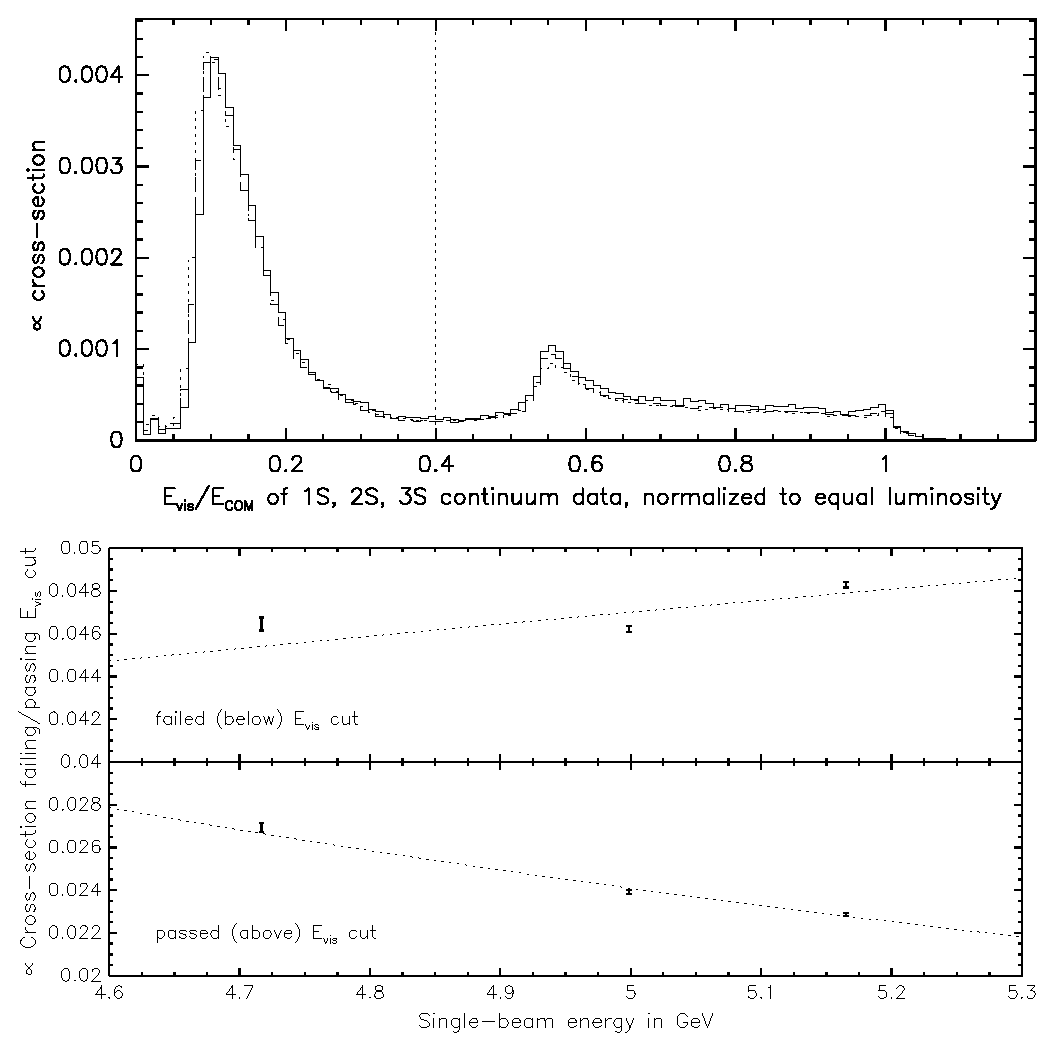
\includegraphics[width=\linewidth]{plots/datasets_twophoton_visen}
  \end{center}
  \caption{\label{datasets:visen_continuum} Top: visible energy from
    unfiltered continuum datasets below $\Upsilon(1S)$,
    $\Upsilon(2S)$, and $\Upsilon(3S)$, with other hadron cuts applied
    except \lfourdec, normalized to equal luminosity using bhabhas.
    Bottom: the integral of the histogram from 0 to 0.4 (``failed
    (below) \visen\ cut'') and from 0.4 to 1.2 (``passed (above)
    \visen\ cut'') versus beam energy.  In each case, $a \log s + b/s$
    has been fit to the points.}
\end{figure}

If I fit the expression
\begin{equation}
  a \log s + b/s \label{datasets:visen_continuum_fitfunc}
\end{equation}
to these three points, I obtain $a/(a+b)$ of 47\% (with an
unbelievable $\chi^2$).  However, if I leave out the first few bins in
\visen, $a/(a+b)$ drops to 17\% (though the three cross-sections still
monotonically increase).  The fit is probably being pulled by unequal
cosmic ray and beam-gas backgrounds in the three continuum datasets.

If I fit the same expression to events that pass the \visen\ cut
(bottom of Figure \ref{datasets:visen_continuum}), $a/(a+b)$ is
0.15\%, negligibly small.  Also, the $\chi^2$ of this fit is 5.8,
which is marginally consistent with one degree of freedom (2\%
confidence level).  From later studies, I know that 1--2\% of the
events that pass the hadron cut can be cosmic rays; inserting
backgrounds on this scale by hand at worst doubles $a/(a+b)$.
Therefore, two-photon backgrounds are negligible after hadron cuts and
the continuum subtraction.

The other backgrounds to be subtracted are beam-gas and cosmic rays.
After the continuum subtraction, it is possible that these backgrounds
have a negative contribution, since the continuum dataset may contain
more beam-gas or cosmic rays than the signal dataset.  Continuing the
technique of subtracting the most heterogeneous control samples first,
the next background to go is beam-gas, because the single-beam
datasets contain cosmic rays.  Here, the scale factors $S_{e^-}$ and
$S_{e^+}$ are the ratios of beam-gas events in the
continuum-subtracted signal to beam-gas events in the single-beam
datasets.  This subtraction is illustrated in Figure
\ref{datasets_beamgas}: beam-gas events are selected in the signal
dataset and in the control dataset, and the control dataset is
normalized to have equal beam-gas.  Note that the beam-gas fraction is
nearly proportional to integrated luminosity, because after the
continuum subtraction, there is little beam-gas left (except for a
little positron-induced beam-gas in the $\Upsilon(2S)$).  This is
another correction whose uncertainty will be taken to be all of
itself.

\begin{figure}[p]
  \begin{center}
    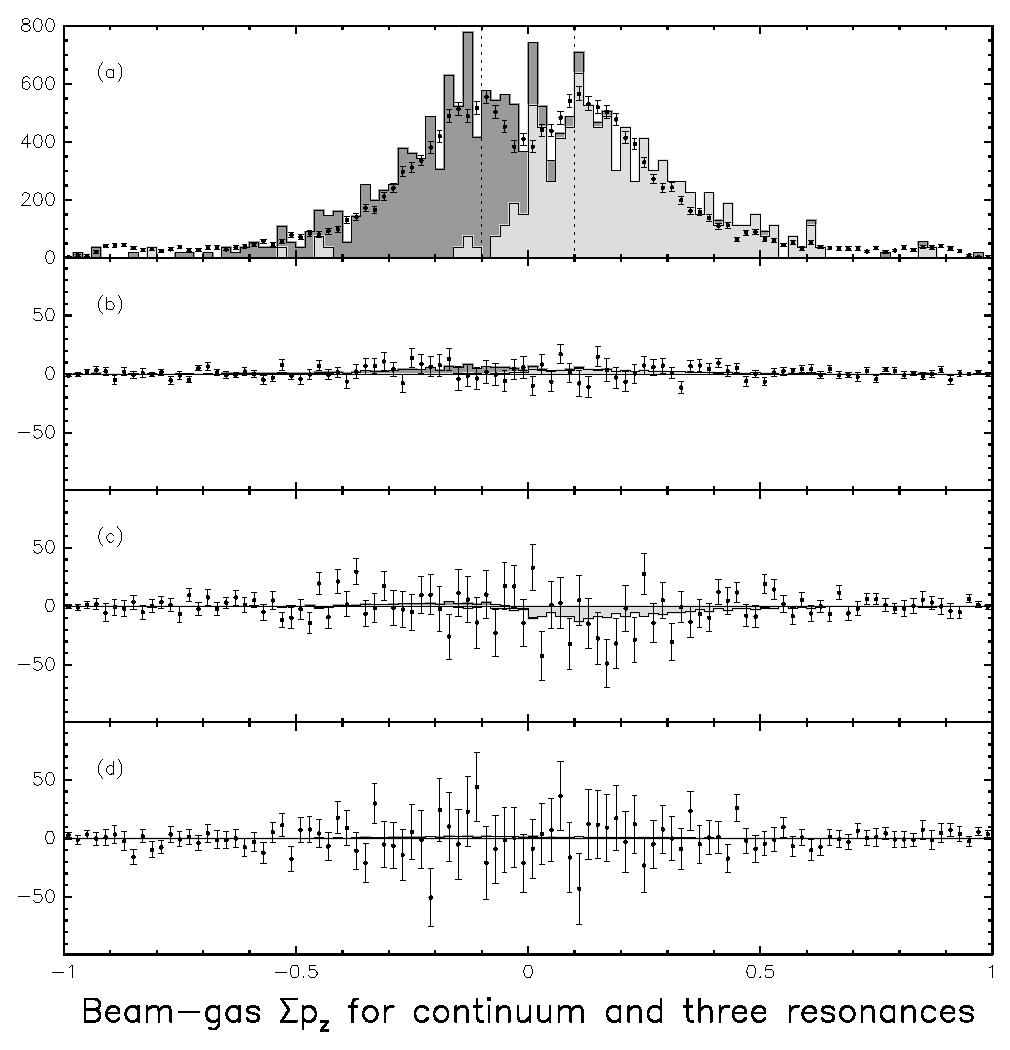
\includegraphics[width=\linewidth]{plots/datasets_beamgas}
  \end{center}
  \caption{\label{datasets_beamgas} Net Z momentum / \ebeam\ from the
    unfiltered dataset, after other beam-gas cuts, in four cases, top
    to bottom: (a) sum of all continuum, (b) continuum-subtracted
    $\Upsilon(1S)$, (c) continuum-subtracted $\Upsilon(2S)$, and (d)
    continuum-subtracted $\Upsilon(3S)$.  The lightly-shaded histogram
    is from positron single-beam and the darker histogram stacked on
    top of it is from electron single-beam.  Dotted lines in
    sub-Figure (a) indicate beam-gas cuts.}
\end{figure}

Finally, cosmic rays are subtracted in the same way.  Cosmic ray cuts
are applied to signal and no-beam control, and $S_0$ is taken to be
their ratio.  This subtraction is illustrated in Figure
\ref{datasets_cosmic}.

Monte Carlo with all $\Upsilon$ decays should look like the unfiltered
data with continuum, beam-gas, and cosmic rays subtracted.

\begin{figure}[p]
  \begin{center}
    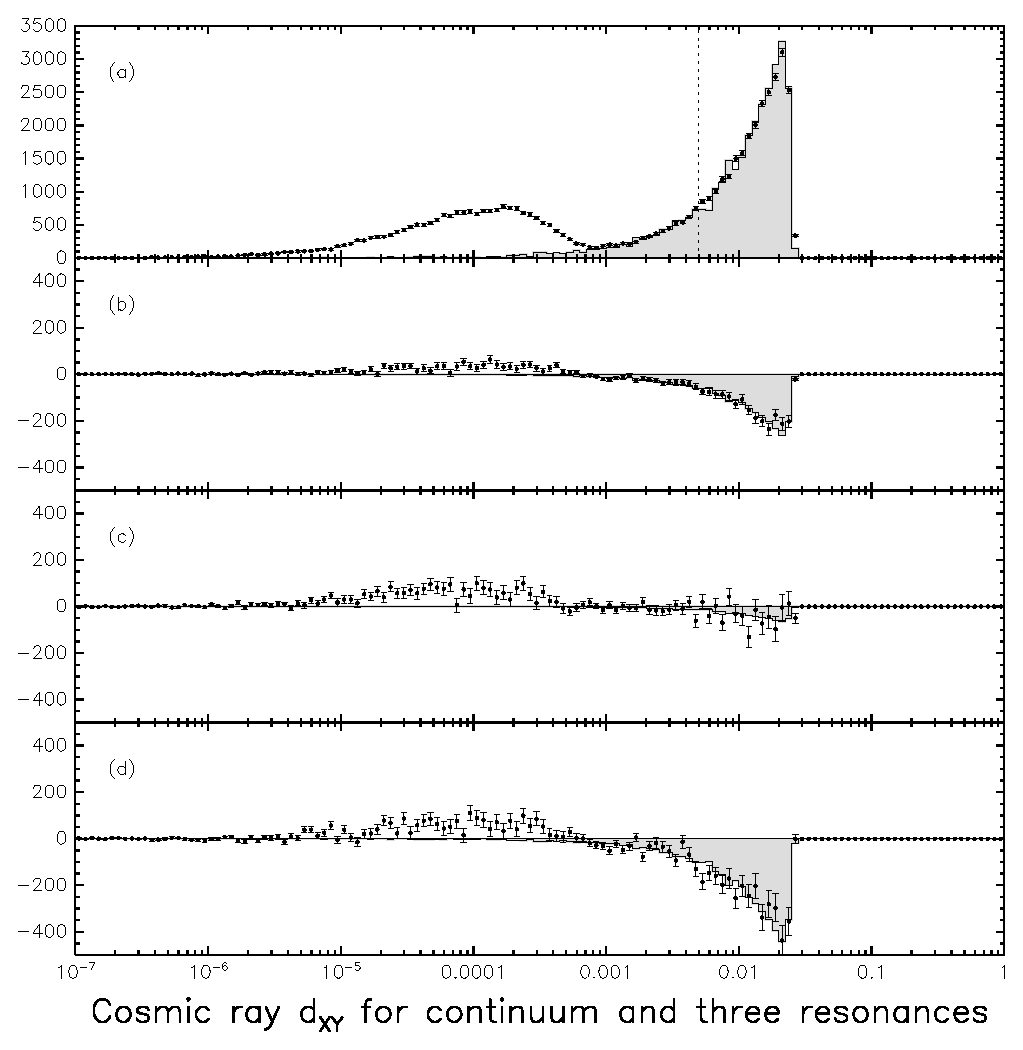
\includegraphics[width=\linewidth]{plots/datasets_cosmic}
  \end{center}
  \caption{\label{datasets_cosmic} Closest track to beam spot XY, in
    log $x$ scale, after other cosmic ray cuts.  The four cases are,
    from top to bottom: (a) sum of all continuum, (b) continuum- and
    beam-gas-subtracted $\Upsilon(1S)$, (c) same for $\Upsilon(2S)$,
    and (d) same for $\Upsilon(3S)$.  The shaded histogram is from the
    no-beam sample, and the dotted line is the cosmic ray cut.  The
    cosmic ray ``peak'' in log $x$ is a flat background in linear $x$.
    The units are meters (so 0.01 is a centimeter, etc.).}
\end{figure}

\section{Scale Factors in the Database Dataset}

The database dataset will be used for lineshape fitting, and I would
rather leave the continuum in the hadron count and fit to it as a
parameter than to subtract it explicitly (and therefore need to
explicitly propagate its uncertainty).  However, beam-gas and cosmic
rays can vary from run to run, so they still must be subtracted
explicitly.

As mentioned above, luminosity will be measured in the database
dataset by counting gamgam events.  Gamgams scale as $1/s$, so the
scale factor for converting hadron counts into something proportional
to hadronic cross section is
\begin{equation}
  S_c^{\mbox{\scriptsize database}} = \mbox{\# gamgams on-res} /
  \mbox{\# gamgams off-res} \times (s_\subs{off-res} /
  s_\subs{on-res})\mbox{.}
\end{equation}
The lineshape fits will be performed after all hadron cuts have been
applied, so the two-photon background is negligible.

As for beam-gas and cosmic rays, we are only interested in how many
survive the hadron cuts.  Passing the no-beam sample through hadron
cuts tells us how many cosmic rays survive (provided that I scale the
no-beam sample to have the same number of cosmic rays as a given run
number), but doing the equivalent thing for beam-gas requires first
removing the cosmic rays from the single-beam samples.  To express
this symbolically,
\begin{flushright}
  \begin{tabular}{r c p{0.7\linewidth}}
    $H_x$, $C_x$, $E_x$, $P_x$ &=& \#events surviving hadron, cosmic
    ray, electron beam-gas, or positron beam-gas, respectively, from
    dataset $x$ \\
  \end{tabular}
  \begin{tabular}{r c p{0.7\linewidth}}
    $x$ &\mbox{ }& can be no-beam, $e^-$-beam, $e^+$-beam, or run, for a
    given run number to be studied \\
  \end{tabular}
  \begin{tabular}{r c p{0.7\linewidth}}
    $N_C$, $N_E$, $N_P$ &=& \#events surviving hadron cuts in
    that run which are really cosmic rays, electron beam-gas, or
    positron beam-gas, respectively.
  \end{tabular}
\end{flushright}
\begin{eqnarray}
  N_C &=& H_\subs{no-beam} \times C_\subs{run} / C_\subs{no-beam}
  \label{datasets_N_C} \\
  N_E &=& (H_\subs{$e^-$-beam} - H_\subs{no-beam} \times
  C_\subs{$e^-$-beam} / C_\subs{no-beam}) \times E_\subs{run} /
  E_\subs{$e^-$-beam} \label{datasets_N_E} \\
  N_P &=& (H_\subs{$e^+$-beam} - H_\subs{no-beam} \times
  C_\subs{$e^+$-beam} / C_\subs{no-beam}) \times P_\subs{run} /
  P_\subs{$e^+$-beam} \label{datasets_N_P}
\end{eqnarray}

The first step in this process (the parenthesized parts of Equations
\ref{datasets_N_E} and \ref{datasets_N_P}) is illustrated in Figure
\ref{datasets:cosmicscale}, where it is also shown that there is very
little feed-through between the beam-gas and cosmic ray cuts.  The
results of these counts, for every run in the database dataset, are
presented in Figure \ref{datasets_databasecontamination}.  For clarity
they are presented as a fraction of the number of continuum
hadrons: if these levels were perfectly flat, there would be no need
to apply any correction, because the backgrounds would be subtracted
along with the continuum.

Beam-gas is a small correction, and it isn't clear how much
non-beam-gas data feeds into the beam-gas cuts (see Figure
\ref{datasets:dxydzcuts}-b).  Therefore, I will apply 50\% $\pm$ 50\%
of the correction.  For a typical run, this means that 0.15\% is
subtracted from the number of hadrons and 0.15\% is added to its
uncertainty.  Cosmic rays are a bigger correction, and the cosmic ray
count represents the number of true cosmic rays to at least 7\% of
itself (see Figure \ref{datasets:dxydzcuts}-a), so the full cosmic ray
correction is applied to each run, propagating only statistical
errors.  Counting statistics from the no-beam sample (which is a 7\%
uncertainty) apply to the whole dataset uniformly, but that can't make
more than a 1\% $\times$ 7\% = 0.07\% difference in the total hadron
count.  I'll just take 0.07\% as a systematic error on $\Gamma_{ee}$.

\begin{figure}[p]
  \begin{center}
    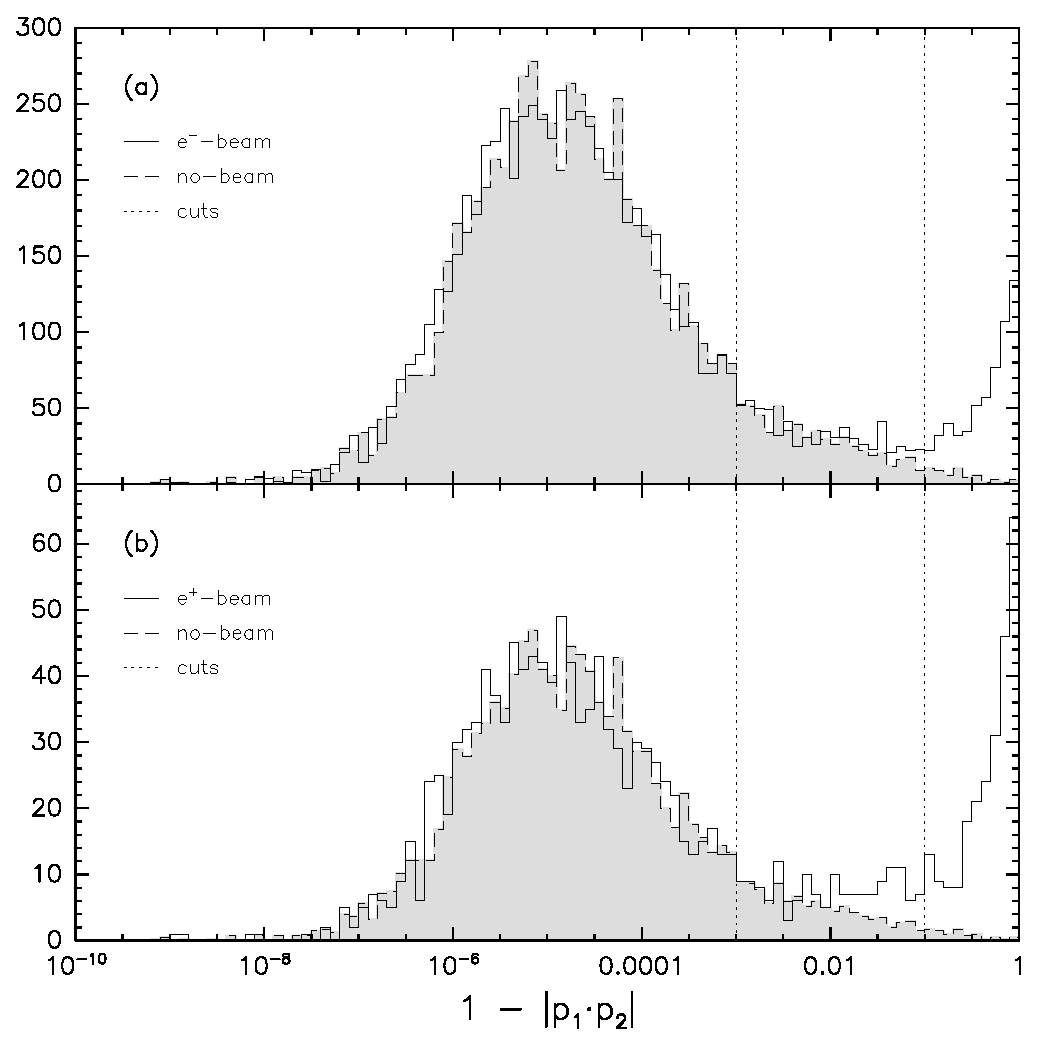
\includegraphics[width=\linewidth]{plots/datasets_cosmicscale}
  \end{center}
  \caption{\label{datasets:cosmicscale} Cosmic-ray back-to-backness
    parameter 1 $-$ \pdotp, in log $x$ scale, after other cosmic ray
    cuts.  Top (a) is electron single-beam and bottom (b) is positron
    single-beam; both are overlaid with the same no-beam sample
    (shaded).  Back-to-back cosmic rays peak around $10^{-5}$, but
    randomly-oriented beam-gas events ``peak'' near 1.  (They are flat
    in linear $x$.)}
\end{figure}

\begin{figure}[p]
  \begin{center}
    \includegraphics[width=\linewidth]{plots/datasets_databasecontamination}
  \end{center}
  \caption{\label{datasets_databasecontamination} Non-beam interaction
    backgrounds that survive hadron cuts ($N_C$, $N_E$, and $N_P$) as
    a percentage of continuum hadrons.  Top to bottom: (a) cosmic
    rays, (b) electron beam-gas, and (c) positron beam-gas.  Dotted
    lines separate $\Upsilon(3S)$, $\Upsilon(1S)$, and $\Upsilon(2S)$
    (from left to right).  Runs used in the unfiltered dataset are
    circled.}
\end{figure}

\begin{figure}[p]
  \begin{center}
    \includegraphics[width=\linewidth]{plots/datasets_database_dxydzcuts}
  \end{center}
  \caption{\label{datasets:dxydzcuts} Geometry cuts which distinguish
    cosmic rays and beam-gas from beam-beam collision data.  Top to
    bottom: (a) closest track to the beam spot in XY for all database
    data (solid histogram) overlaid by no-beam sample (points), with
    other cosmic ray cuts applied, (b) Z of primary vertex for all
    database data (solid histogram) overlaid by a sum of the
    single-beam samples (points), with other beam-gas cuts applied.
    Both are in log $x$ scale with units of meters.}
\end{figure}
